
In this paper, we study issues of scalability of parallel solvers of
the satisfiability (SAT) problem on hierarchical-memory multicore
(SMP) systems. We find this topic important for three reasons.

Since at least 2009, parallel SAT solvers (henceforth, pSATs) have
been performing at the top of the SAT Competition (in 2011, all three
wall-clock time winners of the competition are parallel solvers).
Also in 2011, pSATs and sequential SAT solvers are grouped into a
single competition
track\footnote{\url{http://www.satcompetition.org/}}, which signals
the widespread interest in pSATs by the research and industrial
communities. This appeal stems in part because of the inherent
interesting properties of parallel algorithms, but also because of the
need of the community to do better in other application domains and be
able to handle even larger and more complex CNF formulas in smaller
times taking advantage of modern hardware.

Meanwhile, instead of increasing clock performance, chip manufacturers
are investing heavily on multicore architectures to improve
performance and lower power consumption (AMD released the 8-core
Opteron 3260 EE in late 2011, and Intel will do the same with the Xeon
E5-2650, and its low power version, the Xeon E5-2650L early this
year). As Herb Sutter once put it, ``the free lunch is over''
\cite{FreeLunchIsOver}, and this has effectively meant that software
in general will not be getting any faster as years go by simply
relying on faster processors, but by relying on how software scales in
multicore systems.

Finally, modern memory architectures are not flat
Processor$\leftrightarrow$RAM architectures, but a hierarchy of
faster-but-smaller to slow-but-large memories with latencies varying
from 0.5{\it ns} access, 32{\it Kb} memories such as the L1 cache, to
tens of nanoseconds, megabyte-large memories like the L3 cache, to
gigabyte, 100{\it ns} access memory such as main memory. Hierarchical
memory architectures have a strong impact on the performance of
sequential software (e.g., row scanning arrays in row-major
representation, memory transfers may be in the order of the input
divided by the size of the cache line, while memory transfers for
column scanning is in the order of the square of the input). % For
% multicore systems, besides the problem of data representation, there
% is the problem of false sharing: if two threads write on different
% words of the same cache line, then the cache line in one or the other
% processor becomes ``dirty'' and a round trip to RAM ensues, wasting
% valuable time due to latency.

Thus, given the three arguments above: how {\em do} pSATs scale in
hierarchical-memory multicore architectures? Our case study is the
winner of the 2011 SAT Competition, {\tt plingeling}, a
portfolio-approach SAT solver \cite{lingeling}. The first experiment
tested a \emph{modified} \pling\ on a 6-core multicore machine,
varying the number of threads. This instance of \pling\ was modified
in order that, for each {\em worker thread}, the {\em same search}
would be performed (i.e. same strategies, starting parameters and
without lemma exchanging). This allows us to measure the impact of
running $p$ threads on the same physical CPU. In Figure
\ref{fig:decay} we can see now how the modified-\pling's performance
tends to decay sharply (up to 30\%) when several instances are
executed on the same processor, even when they do not, in principle,
share any resources other than the common process address space. We
would thus expect that all instances would perform similarly, plus or
minus a small time fraction. This is in fact what happens when \pling\
is run in two different cores of two different chips, in different
and even in the same machine.

\begin{figure}[tp]
  \centering
  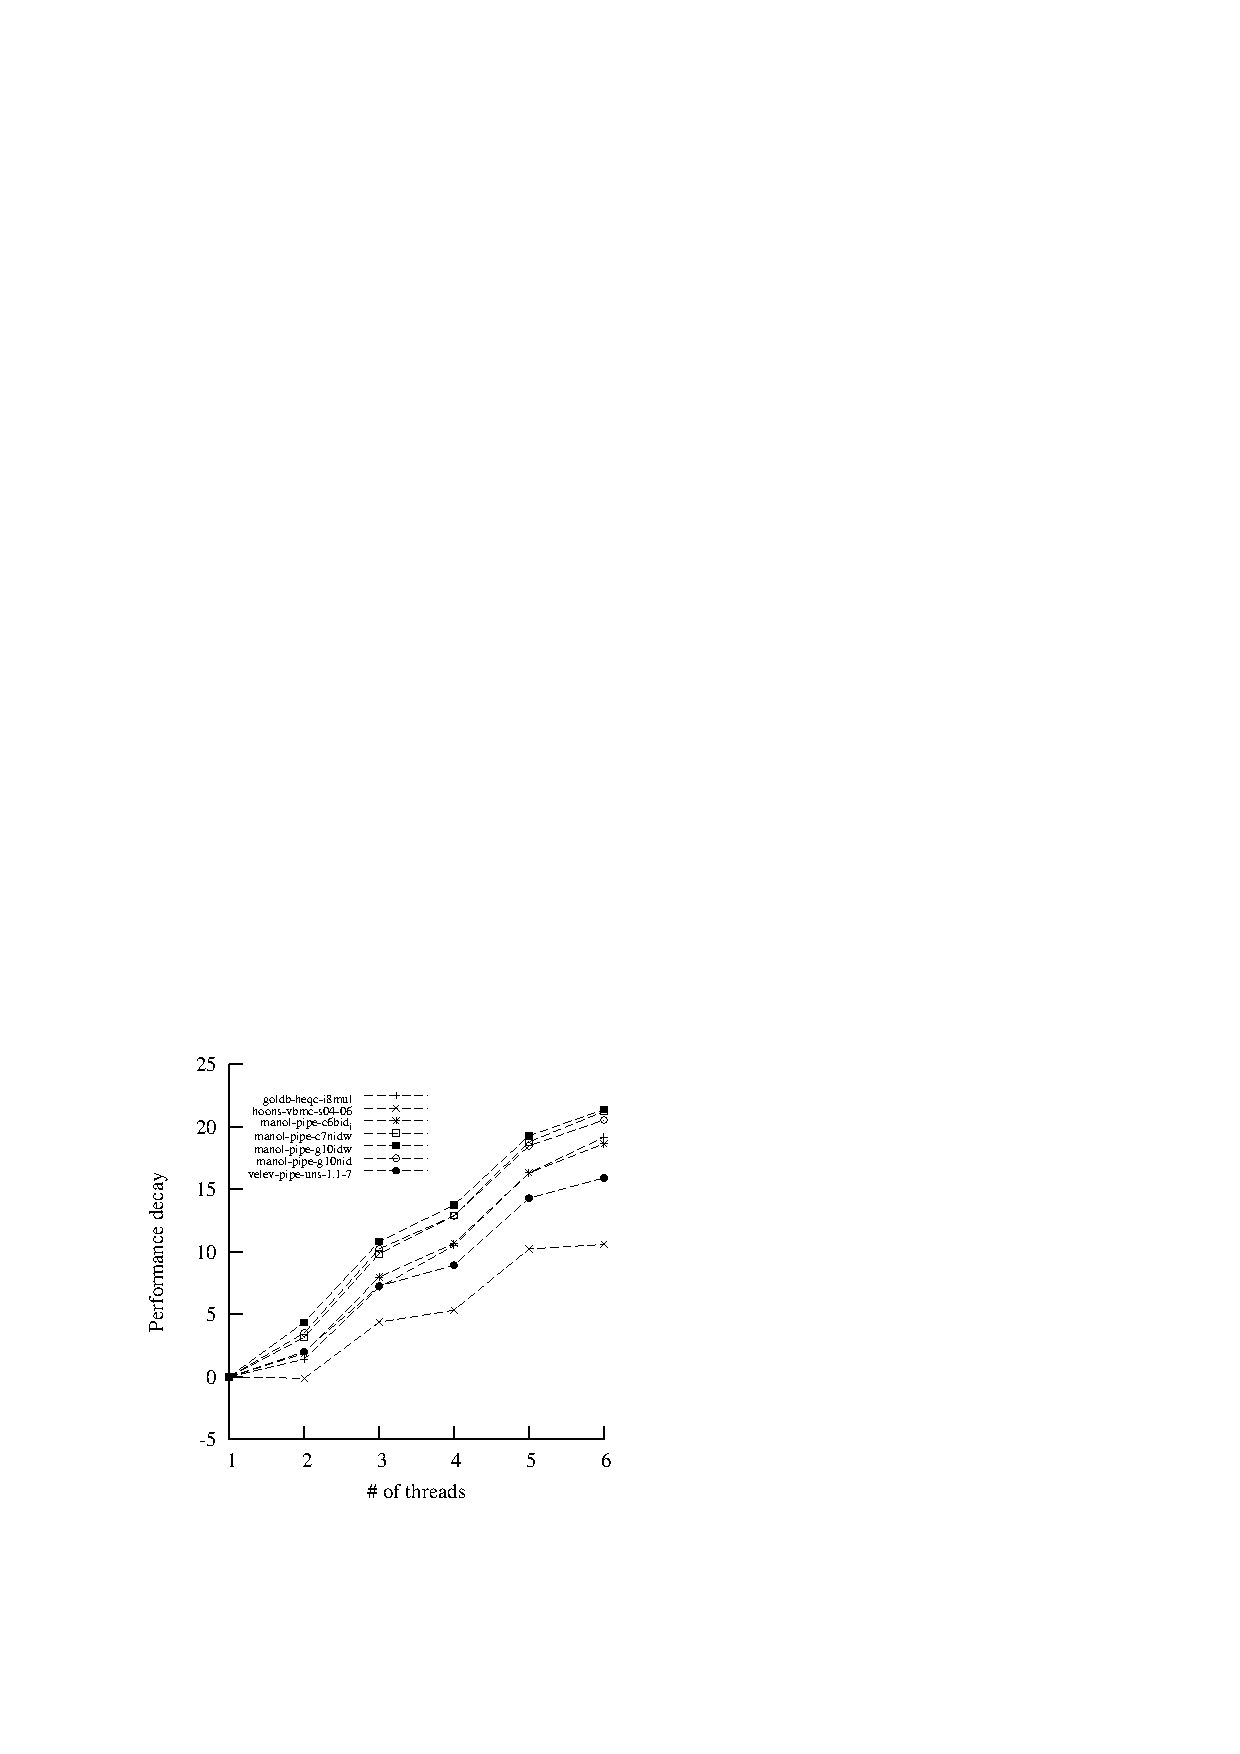
\includegraphics[scale=1]{plingeling_6cores_speedup}
  \caption{Performance decay of {\tt plingeling} when run over many cores}
  \label{fig:decay}
\end{figure}

In order to find the reason of the performance decay, we have
developed a simple portfolio-approach-based SAT solver (which we have
called AzuDICI) that allows us to both replicate the behavior of
\pling, and then also experiment with alternative scenarios (such as
sharing information among threads) in order to take measures towards
the improvement of its performance. It is important to highlight that
our SAT solver does not compare to high-performance current
state-of-the-art solvers such as \pling\ itself. AzuDICI serves as a
useful tool to test and analyze the behavior of
portfolio-approach-based SAT solvers.

%In Section \ref{} we.....

%%% Local Variables: 
%%% mode: latex
%%% TeX-master: t
%%% End: 
